\documentclass{article}
\usepackage[margin=1in]{geometry}
\usepackage{amsmath,amsthm,amssymb}
\usepackage{bbm,enumerate,mathtools}
\usepackage{tikz,pgfplots}
\usepackage{chessboard}
\usepackage[hidelinks]{hyperref}
\usepackage{multicol} % Problem 35
\usepackage{xstring} % Difficulty command
\usetikzlibrary{shapes.geometric}

\newenvironment{question}{\begin{trivlist}\item[\textbf{Question.}]}{\end{trivlist}}
\newenvironment{note}{\begin{trivlist}\item[\textbf{Note.}]}{\end{trivlist}}
\newenvironment{references}{\begin{trivlist}\item[\textbf{References.}]}{\end{trivlist}}
\newenvironment{related}{\begin{trivlist}\item[\textbf{Related.}]\end{trivlist}\begin{enumerate}}{\end{enumerate}}

\newcommand\score[1]{
\pgfmathsetmacro\pgfxa{#1+1}
\tikzstyle{scorestars}=[
  star,
  star points=5,
  star point ratio=2.25,
  draw,
  inner sep=3pt,
  anchor=outer point 5
]
  \begin{tikzpicture}[baseline]
    \draw[opacity=0] (0,-0.5) rectangle (0,0.2); % Workaround for whitespace at the bottom.
    \foreach \i in {1,...,4} {
      \pgfmathparse{(\i<=#1?"yellow":"gray")}
      \edef\starcolor{\pgfmathresult}
      \draw (\i*4.5ex,0) node[name=star\i,scorestars,fill=\starcolor]  {};
    }
  \end{tikzpicture}
}

\newcommand{\difficulty}[1]{%
  \IfEqCase{#1}{%
      {1}{
        
\begin{tikzpicture}[scale=0.7, baseline=0.9mm]%
          \definecolor{slopegreen}{rgb}{0.0, 0.5, 0.0}%
          \fill[slopegreen] (0.5,0.5) circle (0.5);%
        \end{tikzpicture}%
      }%
      {2}{
        
\begin{tikzpicture}[scale=0.7, baseline=0.9mm]%
          \definecolor{slopeblue}{rgb}{0.0, 0.44, 1.00}
          \fill[slopeblue] (0,0) rectangle (1,1);%
        \end{tikzpicture}%
      }%
      {3}{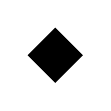
\begin{tikzpicture}[scale=0.7, baseline=0.9mm]\fill (0,0.5)--(0.5, 0)--(1,0.5)--(0.5,1)--cycle; \end{tikzpicture}}%
      {4}{
\begin{tikzpicture}[scale=0.7, baseline=0.9mm]\fill (0.25,0)--(0,0.5)--(0.25,1)--(0.5,0.5)--cycle; \fill (0.75,0)--(0.5,0.5)--(0.75,1)--(1,0.5)--cycle;\end{tikzpicture}}%
      % you can add more cases here as desired
  }[\PackageError{difficulty}{Undefined difficulty level: #1}{}]%
}%
\newcommand{\rating}[2]{\difficulty{#1}\\\score{#2}\\}


\begin{document}
\rating{3}{2}
A hyperbolic $\mathrm{poly}_{\{p,k\}}$-form is a polyform on the hyperbolic plane that
consists of $p$-gons on the tiling of the hyperbolic plane with Schl\"afli
symbol $\{p,k\}$.
A hyperbolic polyform with $n$ cells is called a hyperbolic $n_{\{p,k\}}$-form.

\begin{figure}[ht!]
  \centering
  \includegraphics[scale=0.15]{assets/120_problem/5_4_hyperbolic_polyominoes.pdf}
  \caption{
    The $A119611(5)$ free pentominoes in the tessellation of the
    hyperbolic plane with Schl\"afli symbol $\{5,4\}$.
  }
\end{figure}

\begin{question}
  What is the asymptotic growth of $n_{\{p,k\}}$-form as a function of $n$,
  the number of cells?
\end{question}

\begin{related}
  \item Can this generalize to three or more dimensions the way polyominoes
  generalize to polycubes?
  \item Is there a meaningful notion of fixed vs 1-sided
    $\mathrm{poly}_{\{p,k\}}$-forms?
\end{related}


\begin{references}
  \item Problems 71, 72, 77, 101, 103, 108, and 109.
  \item \href{https://codegolf.stackexchange.com/q/200122/53884}{Code Golf Stack Exchange: Counting polyominoes on the hyperbolic plane.}
  \item \href{https://arxiv.org/abs/2109.05331}{arXiv: Extremal $\{p,q\}$-Animals}
\end{references}
\end{document}
